

\section{Motivation}
\begin{frame}
\frametitle{\centering Optimization under uncertainity}
\begin{small}
\begin{block}{}
\begin{columns}[T]
\begin{column}{.48\textwidth}
\color{red}\rule{\linewidth}{4pt}
Energy Demand management
\begin{itemize}
\item Consumer demand, energy generation are uncertain.
\item Objective is to minimize the difference.
\end{itemize}
\end{column}
\begin{column}{.48\textwidth}
\begin{figure}

\includegraphics[width=5cm,height=3cm]{energymgmt}
\end{figure}
\end{column}
\end{columns}
\end{block}
\begin{block}{}
\begin{columns}[T]
\begin{column}{.48\textwidth}
\color{blue}\rule{\linewidth}{4pt}
Traffic signal control
\begin{itemize}
\item Optimal order to switch traffic lights.
\item Objective is to minimize waiting time.
\end{itemize}
\end{column}
\begin{column}{.48\textwidth}
\begin{figure}
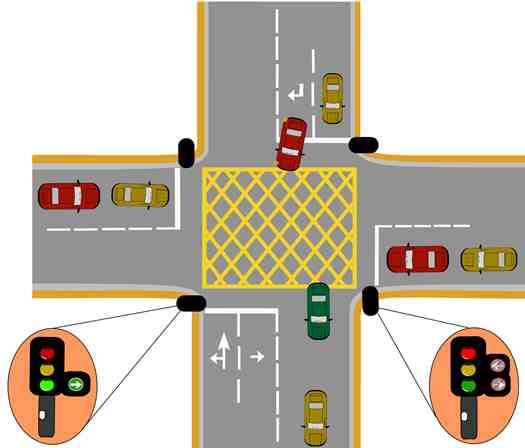
\includegraphics[width=4cm,height=2.7cm]{traffic}
\end{figure}
\end{column}
\end{columns}
\end{block}

\end{small}
\end{frame}




%\begin{frame}
%\frametitle{\centering Motivation}
%\begin{block}{}
%
%\begin{itemize}
%\item Communication networks
%\begin{itemize}
%\item To optimally allocate link bandwidth amongst competing traffic flows.
%\end{itemize}
%\item Vehicular traffic network
%\begin{itemize}
%\item To find the optimal order to switch traffic lights at  junctions .
%\end{itemize}
%\item Manufacturing systems
%\begin{itemize}
%\item To decide the optimal order in which to allocate machine capacity for manufacturing various products.
%\end{itemize}
%
%\item Economics
%\end{itemize}
%\end{block}
%\end{frame}


\section{Introduction }
%\subsection{Classification of optimization problems}
\begin{frame}
\frametitle{\centering Basic optimization problem}
\begin{block}{}
\begin{small}
To find $\theta^{*}$ that minimizes the objective function $f(\theta)$ :
\begin{align}\label{eq:opt}
 \theta^* = \underset{\theta \in \Theta}{\argmin} ~f(\theta),
\end{align}
\end{small}
\end{block}
\begin{small}
\begin{itemize}
\item $f \colon \mathbb{R}^N \to \mathbb{R}$ is called the objective function.
\item $\theta$ is tunable N-dimensional parameter
\item $\Theta \subseteq \mathbb{R}^N$ is the constraint set in which $\theta$ takes values.
\end{itemize}
\end{small}
\end{frame}

\begin{frame}
\frametitle{\centering Based on  objective function}
\begin{small}
\begin{columns}[T]
\begin{column}{.48\textwidth}
\color{red}\rule{\linewidth}{4pt}
Deterministic optimization problem
\begin{itemize}
\item Complete information about objective function $f$.
\item First and higher order derivatives.
\item Set $\Theta$.
\end{itemize}
\end{column}
\begin{column}{.48\textwidth}
\color{blue}\rule{\linewidth}{4pt}
Stochastic optimization problem
\begin{itemize}
\item We have little knowledge on the structure of $f$.
\item $f$ cannot be obtained directly.
\item $f(\theta) \equiv E_{\xi}[h(\theta,\xi)]$, where $\xi$ comprises the randomness in the system.
\end{itemize}
Complex  to find $\theta^{*}$ only on the basis of noisy samples.
\end{column}
\end{columns}
\end{small}
\end{frame}

%\begin{frame}
%\frametitle{\centering Based on feasible region}
%\begin{block}{}
%Based on structure of feasible region $\Theta$, optimization problems can be classified into:
%\begin{itemize}
%\item Continuous
%\item Discrete
%\item Hybrid
%\end{itemize}
%\end{block}
%\end{frame}

\section{Optimization via Simulation}

\begin{frame}
\frametitle{\centering  Stochastic optimization via simulation}
\begin{small}
\begin{block}{}
Stochastic optimization deals with  highly nonlinear and high dimensional systems. The challenges with these problems are:
\begin{itemize}
\item Too complex to solve analytically.
\item Many simplifying assumptions are  required.
\end{itemize}
\end{block}
\begin{block}{}
A good alternative of modelling and analysis is \textbf{"Simulation"}
\end{block}
\begin{block}{Function measurements}
\tikzstyle{block} = [draw, fill=white, rectangle,
   minimum height=3em, minimum width=6em]
\tikzstyle{sum} = [draw, fill=white, circle, node distance=1cm]
\tikzstyle{input} = [coordinate]
\tikzstyle{output} = [coordinate]
\tikzstyle{pinstyle} = [pin edge={to-,thin,black}]

 \begin{figure}[t]
    \centering
\scalebox{0.8}{\begin{tikzpicture}[auto, node distance=2cm,>=latex']
% We start by placing the blocks
\node (theta) {$\boldsymbol{\theta_n}$};
\node [block, fill=blue!20,right=0.6cm of theta,align=center] (sample) {\makecell{\textbf{Simulator}}}; 
\node [right=0.6cm of sample] (end) {$\boldsymbol{\mathbf{f(\theta_n) + \xi_n}}$};
\node [ above right= 0.6cm of end] (bias) {\textbf{Zero mean}};
\draw [->] (theta) --  (sample);
\draw [->] (sample) -- (end);
\path [darkgreen,->] (bias) edge [bend left] (end);
\end{tikzpicture}}
\caption{Simulation optimization}
\label{fig:so}
\end{figure}

\end{block}
\end{small}
\end{frame}




%\begin{frame}
%\frametitle{\centering  Discrete optimization via simulation}
%\begin{block}{}
%\begin{itemize}
%\item $\theta \in \Theta$ is discrete and integer ordered.
%\item $\Theta$ is a subset of $N$-dimensional integers.
%\item $\theta$ can take only countable (finite or infinite) number of values.
%\item Discrete optimization problems are some times called as \emph{combinatorial optimization} problems.
%\end{itemize}
%\end{block}
%\begin{block}{}
%Applications in Resource allocation, Network routing, Policy planning etc.
%\end{block}
%\end{frame}
%
%
%\begin{frame}
%\frametitle{\centering  Sub-classes of DOvS}
%\begin{block}{}
%Consider the case of $\Theta$ being finite i.e., $\Theta = \{\theta_{1},\theta_{2},\ldots,\theta_{k}\}$.
%\begin{itemize}
%\item Two sub-classes of methods are present in the literature based on size of feasible region
%\begin{itemize}
%\item $\Theta$ is small (often less than 100).
%\item $\Theta$ is large 
%\end{itemize}
%\end{itemize}
%\end{block}
%\begin{block}{}
%There are  methods which  allow countably infinite choices for $\theta$.
%\end{block}
%\end{frame}
%
%\begin{frame}
%\frametitle{\centering  $\Theta$ is small}
%\begin{block}{}
%We can simulate all possible solutions and select the best among them. Two popular procedures are:
%\begin{itemize}
%\item Ranking and Selection (R\&S)
%\item Multiple comparison procedures (MCP)
%\end{itemize}
%\end{block}
%\end{frame}
%
%
%\begin{frame}
%\frametitle{\centering  Ranking and Selection (R\&S)}
%\begin{block}{}
%R\&S procedures are statistical procedures.  Majority of work in R\&S is classified into  two categories
%\begin{itemize}
%\item \emph{Indifferent-zone ranking :} Which is aimed  to select the best.
%\begin{itemize}
%\item \emph{The frequentist approach} 
%\item \emph{ Bayesian approach:} One of the popular streams of Bayesian approach procedures is  optimal computing budget allocation (OCBA) 
%\end{itemize}
%
%\item \emph{Subset selection :}  To find subset consisting of best.
%\end{itemize}
%\end{block}
%\end{frame}
%
%\begin{frame}
%\frametitle{\centering The frequentist approach}
%\begin{block}{Bechhofer's procedure }
%Let $\delta$ be indifferent-zone parameter and probability of selecting best solution be $1-\alpha$
%\begin{itemize}
%\item Find $h$ satisfying $Pr\{Z_{i} \leq h, i = 1,2,\ldots,k-1\} = 1-\alpha$. Let $n = \lceil \frac{2h^{2}\sigma^{2}}{\delta^{2}} \rceil$.
%\item Find estimates $\hat{f}(\theta_{i})$ for all $k$ choices
%\item Select the lowest sample mean estimate $\hat{f}(\theta_{i})$ as the best.
%\end{itemize}
%\end{block}
%\end{frame}
%
%\begin{frame}
%\frametitle{\centering  Multiple comparison procedures}
%\begin{block}{}
%Like R\&S, MCPs attempt to identify the best parameter. Three main classes of MCPs   
%\begin{itemize}
%\item \emph{Multiple Comparison approach} (MCA)
%\item \emph{Multiple Comparison with the Best} (MCB)
%\item \emph{Multiple Comparisons with Control} (MCC). 
%\end{itemize}
%\end{block}
%\begin{block}{}
%Simultaneous confidence intervals $J(\theta_{j}) - opt_{i \neq j} J(\theta_{i})$ for $j = 1,2,\ldots,k$ can be used to determine $j_{*}$ for which confidence interval is zero.
%\end{block}
%\end{frame}
%
%\begin{frame}
%\frametitle{\centering  $\Theta$ is large}
%\begin{block}{}
%Enumeration is too expensive to conduct. Need to incorporate search techniques. Two types of approaches
%\begin{itemize}
%\item \emph{Model-based approaches:}   Approaches using \emph{gradient information} with respect to parameter to help the search like in COvS.
%\item \emph{Metaheuristic:} These are gradient free approaches and often called as \emph{Random search algorithms}. 
%\end{itemize}
%\end{block}
%\end{frame}
%
%
%\begin{frame}
%\frametitle{\centering  Random search algorithms}
%\begin{block}{}
%Let $N(\theta)$ denote neighborhood set of $\theta \in \Theta$.
%\begin{itemize}
%\item Select initial configuration $\hat{\theta}_{*}$, set $n_{\hat{\theta}_{*}} = 1$ and $n_{\theta} = 0$ $\forall \theta \neq \hat{\theta}_{*}$.\\
%\item Iterate : 
%\begin{itemize}
%\item Select $\theta_{i} \in N(\hat{\theta}_{*})$ according to some probability distribution 
%\item Perform simulations to obtain estimates $\widehat{f}(\hat{\theta}_{*})$ and $\widehat{f}(\theta_{i})$.
%\item Increase the counter for best estimate and update the current point
%\begin{itemize}
%\item $n_{\hat{\theta}_{*}} = n_{\hat{\theta}_{*}} + \mathbbm{1}_\{\widehat{f}(\hat{\theta}_{*}) \leq \widehat{f}(\theta_{i})\}$
%\item $n_{\hat{\theta}_{i}} = n_{\hat{\theta}_{i}} + \mathbbm{1}_\{\widehat{f}(\hat{\theta}_{*}) > \widehat{f}(\theta_{i})\}$
%\item If  $\widehat{f}(\hat{\theta}_{*}) > \widehat{f}(\theta_{i})$ then $\hat{\theta}_{*} \leftarrow \theta_{i}$
%\end{itemize}
%\end{itemize}
%\item Output $\theta^{*} = \underset{\theta \in \Theta} {argmax}~ n_{\theta}$
%\end{itemize}
%\end{block}
%\begin{block}{}
%A simple version of above algorithm guaranteed to converge globally w.p.1.
%\end{block}
%\end{frame}

%\begin{frame}
%\frametitle{\centering Continuous optimization via simulation}
%\begin{block}{}
%\begin{itemize}
%\item $\theta \in \Theta$ is a vector of continuous decision variables.
%\item $\Theta$ is a convex subset of $\mathcal{R}^N$.
%\item $\theta$ can take uncountably many values.
%\item Applications in Model fitting, Adaptive control, Neural network training, Signal processing etc.
%\end{itemize}
%\end{block}
%\begin{block}{}
%\textbf{Stochastic approximation algorithms} are best suited and most studied methods for solving COvS problems
%\end{block}
%\end{frame}

\begin{frame}
\begin{small}
\frametitle{\centering  Stochastic approximation + Gradient descent}
\begin{block}{Stochastic analog of gradient descent}
\begin{align}\label{saalg}
\theta_{n+1} = \Gamma_{\Theta} \left [\theta_{n} - a_{n} \widehat{\nabla} f(\theta_{n}) \right],
\end{align}

\begin{itemize}
\item $ \widehat{\nabla} f(\theta_{n})$ is an \textbf{noisy} estimate of the gradient $ {\nabla} f(\theta_{n})$.
\item $\{a_{n}\}$ are  \textbf{pre-determined} step-sizes satisfying: $\sum_{n=1}^{\infty} a_{n}  = \infty$,  $\sum_{n = 1}^{\infty} a_{n}^{2} < \infty$.
\item $\Gamma_{\Theta}$ denotes the projection of a point  onto $\Theta$.
\end{itemize}
\end{block}
% \begin{block}{}
% SA algorithm is a stochastic analog of \textbf{gradient decent method}.
% \end{block}
\end{small}
\end{frame}

%\begin{frame}
%\frametitle{\centering  Gradient/Hessian estimation methods}
%\begin{block}{}
%Challenge is to estimate the gradient and/or Hessian of $f$ from function samples.
%\end{block}
%\begin{block}{}
%\begin{itemize}
%\item Finite difference stochastic approximation (FDSA). 
%\item Simultaneous perturbation stochastic approximation (SPSA).
%\item Smoothed functional approximation (SFA).
%\item Random direction stochastic approximation (RDSA).
%\end{itemize}
%\end{block}
%\end{frame}

%\begin{frame}
%\frametitle{\centering  FDSA gradient estimate}
%\begin{block}{Function measurements}
%$y_{ni}^+ = f(\theta_n+\delta_n e_i) + \xi_{ni}^+,\quad y_{ni}^- = f(\theta_n-\delta_n e_i) + \xi_{ni}^-$, $i= 1,2,\ldots,N$
%\end{block}
%\begin{block}{Gradient estimate}
%\begin{align}\label{eq:fdsa}
% \widehat{\nabla} f(\theta_{n}) = \left(
%\begin{array}{c}
%\frac{f(\theta_n+\delta_n e_1)-f(\theta_n-\delta_n e_1)}{2\delta_n} + \frac{\xi_{n}^+ - \xi_{n}^-}{2\delta_n}\\
%\vdots\\
%\frac{f(\theta_n+\delta_n e_N)-f(\theta_n-\delta_n e_N)}{2\delta_n} +  \frac{\xi_{n}^+ - \xi_{n}^-}{2\delta_n}\\
%\end{array}
%\right)
%\end{align}
%\end{block}
%\end{frame}



